\documentclass[11pt,a4paper]{article}

\usepackage[margin=1in]{geometry}
\usepackage{amsmath,amssymb}
\usepackage{lmodern}
\usepackage[T1]{fontenc}
\usepackage[utf8]{inputenc}
\usepackage{booktabs}
\usepackage{tabularx}
\usepackage{graphicx}
\usepackage{microtype}
\usepackage{listings}
\usepackage{xcolor}
\usepackage{lineno}
\usepackage[numbers,sort&compress]{natbib}
\usepackage[colorlinks=true,linkcolor=blue,citecolor=blue,urlcolor=blue]{hyperref}

% Listings configuration for code blocks
\definecolor{codegreen}{rgb}{0,0.6,0}
\definecolor{codegray}{rgb}{0.5,0.5,0.5}
\definecolor{codepurple}{rgb}{0.58,0,0.82}
\definecolor{backcolour}{rgb}{0.96,0.96,0.96}

\lstdefinestyle{mystyle}{
    backgroundcolor=\color{backcolour},   
    commentstyle=\color{codegreen},
    keywordstyle=\color{magenta},
    numberstyle=\tiny\color{codegray},
    stringstyle=\color{codepurple},
    basicstyle=\ttfamily\footnotesize,
    breakatwhitespace=false,         
    breaklines=true,                 
    captionpos=b,                    
    keepspaces=true,                 
    numbers=left,                    
    numbersep=5pt,                  
    showspaces=false,                
    showstringspaces=false,
    showtabs=false,                  
    tabsize=2
}
\lstset{style=mystyle}

\title{\textbf{\Large A Curated and Snapped Geospatial Database of Heavy Metal Concentrations in River Sediments and Waters Across Bangladesh (2010--2024)}}

\author{
    Author One$^{1,*}$, Author Two$^{1,2}$, Author Three$^{2}$ \\[0.5em]
    \small $^{1}$ Department of Environmental Science and Engineering, University Name, Dhaka, 1000, Bangladesh \\
    \small $^{2}$ Institute of Water and Flood Management, Technical University, Dhaka, 1205, Bangladesh \\
    \small $^*$ Corresponding author: \texttt{author.one@university.edu}
}

\date{\today}

\begin{document}

\maketitle
\linenumbers

\begin{abstract}
Potentially toxic heavy metals in riverine corridors of the Ganges-Brahmaputra-Meghna delta threaten aquatic ecology and drinking water security for over 170 million people. Although numerous environmental investigations have been published across Bangladesh over the past 15 years, data remain fragmented in static PDF tables, lack standardized geospatial referencing, and conflate acute dissolved aqueous concentrations with benthic sediment sinks. Here, we present a harmonized, provenance-documented, and hydrologically snapped geospatial database of heavy metal concentrations in river waters and bed sediments across Bangladesh compiled from 28 peer-reviewed publications (2010--2024). The database contains 557 verified analytical assays---289 bed sediment records across 133 unique station centroids and 268 surface water records across 12 major river basins---covering seven key trace elements (As, Cd, Cr, Cu, Ni, Pb, Zn) alongside 106 bulk physicochemical records. All stations are snapped to topological river reach polylines from HydroSHEDS HydroRIVERS (mean offset: 357~m). The database is distributed in open formats (SQLite, CSV, Parquet, GeoPackage) to facilitate regional machine learning, spatial modeling, and water safety planning.
\end{abstract}

\noindent\textbf{Keywords:} Heavy metals; Fluvial water quality; River sediments; Bengal Delta; HydroSHEDS; Open geospatial database

\section*{Background \& Summary}
River networks of developing deltaic nations face acute environmental pressures from rapid industrial expansion, urbanization, and agrochemical runoff. In Bangladesh, situated in the Bengal Delta at the confluence of the Ganges, Brahmaputra, and Meghna rivers, untreated effluents from leather tanneries, textile dyeing mills, metal finishing plants, and municipal discharges are routed directly into natural river corridors \citep{Islam2015,Bhuiyan2015}. Heavy metals and metalloids (e.g., Lead, Chromium, Cadmium, Arsenic, Nickel, Copper, Zinc) represent a premier environmental hazard due to their environmental persistence, potential for trophic bioaccumulation, and chronic human toxicity \citep{Jarup2003,Tchounwou2012}.

Despite substantial academic research on heavy metal pollution in Bangladeshi rivers published between 2010 and 2024, existing datasets suffer from severe fragmentation and usability barriers:
\begin{enumerate}
    \item \textbf{Isolated Static Formats:} Concentration measurements are locked within unstructured tables in supplementary PDFs, preventing automated ingestion, meta-analysis, or large-scale machine learning.
    \item \textbf{Inconsistent Georeferencing:} Published sampling locations often lack verified coordinates, report coordinates in conflicting formats (DMS, decimal degrees, coordinate ranges), or report coordinates that fall on terrestrial landmasses due to typographical errors.
    \item \textbf{Absence of Fluvial Topological Routing:} Environmental mapping studies typically interpolate river water and sediment metals using two-dimensional planar Euclidean methods (such as Ordinary Kriging or Inverse Distance Weighting). However, rivers are directed dendritic networks governed by upstream flow accumulation, catchment topography, and stream order \citep{Lehner2013}. Planar interpolation creates severe boundary artifacts across dry landmasses and between hydrologically disconnected basins.
    \item \textbf{Fraction Confounding:} Existing literature frequently fails to distinguish between dissolved aqueous fractions ($<0.45\ \mu\text{m}$ filtered) and total recoverable digestions, or conflates acute water measurements with decadal sediment repositories.
\end{enumerate}

To overcome these structural limitations, we created a standardized, quality-controlled, and topologically snapped relational database consolidating published heavy metal measurements in Bangladesh rivers from 2010 through 2024. The resulting database synthesizes 557 analytical records across 28 peer-reviewed studies and 12 river systems into a relational SQLite architecture and open CSV/Parquet formats. Every station has been georeferenced and snapped to the nearest reach segment of the global HydroSHEDS HydroRIVERS hydrographic network, pairing chemical concentrations with upstream catchment area, Strahler stream order, annual discharge, and distance to the river mouth. This dataset provides an essential, ready-to-use digital foundation for researchers, environmental regulators, and spatial hydrologists.

\begin{figure}[htbp]
\centering
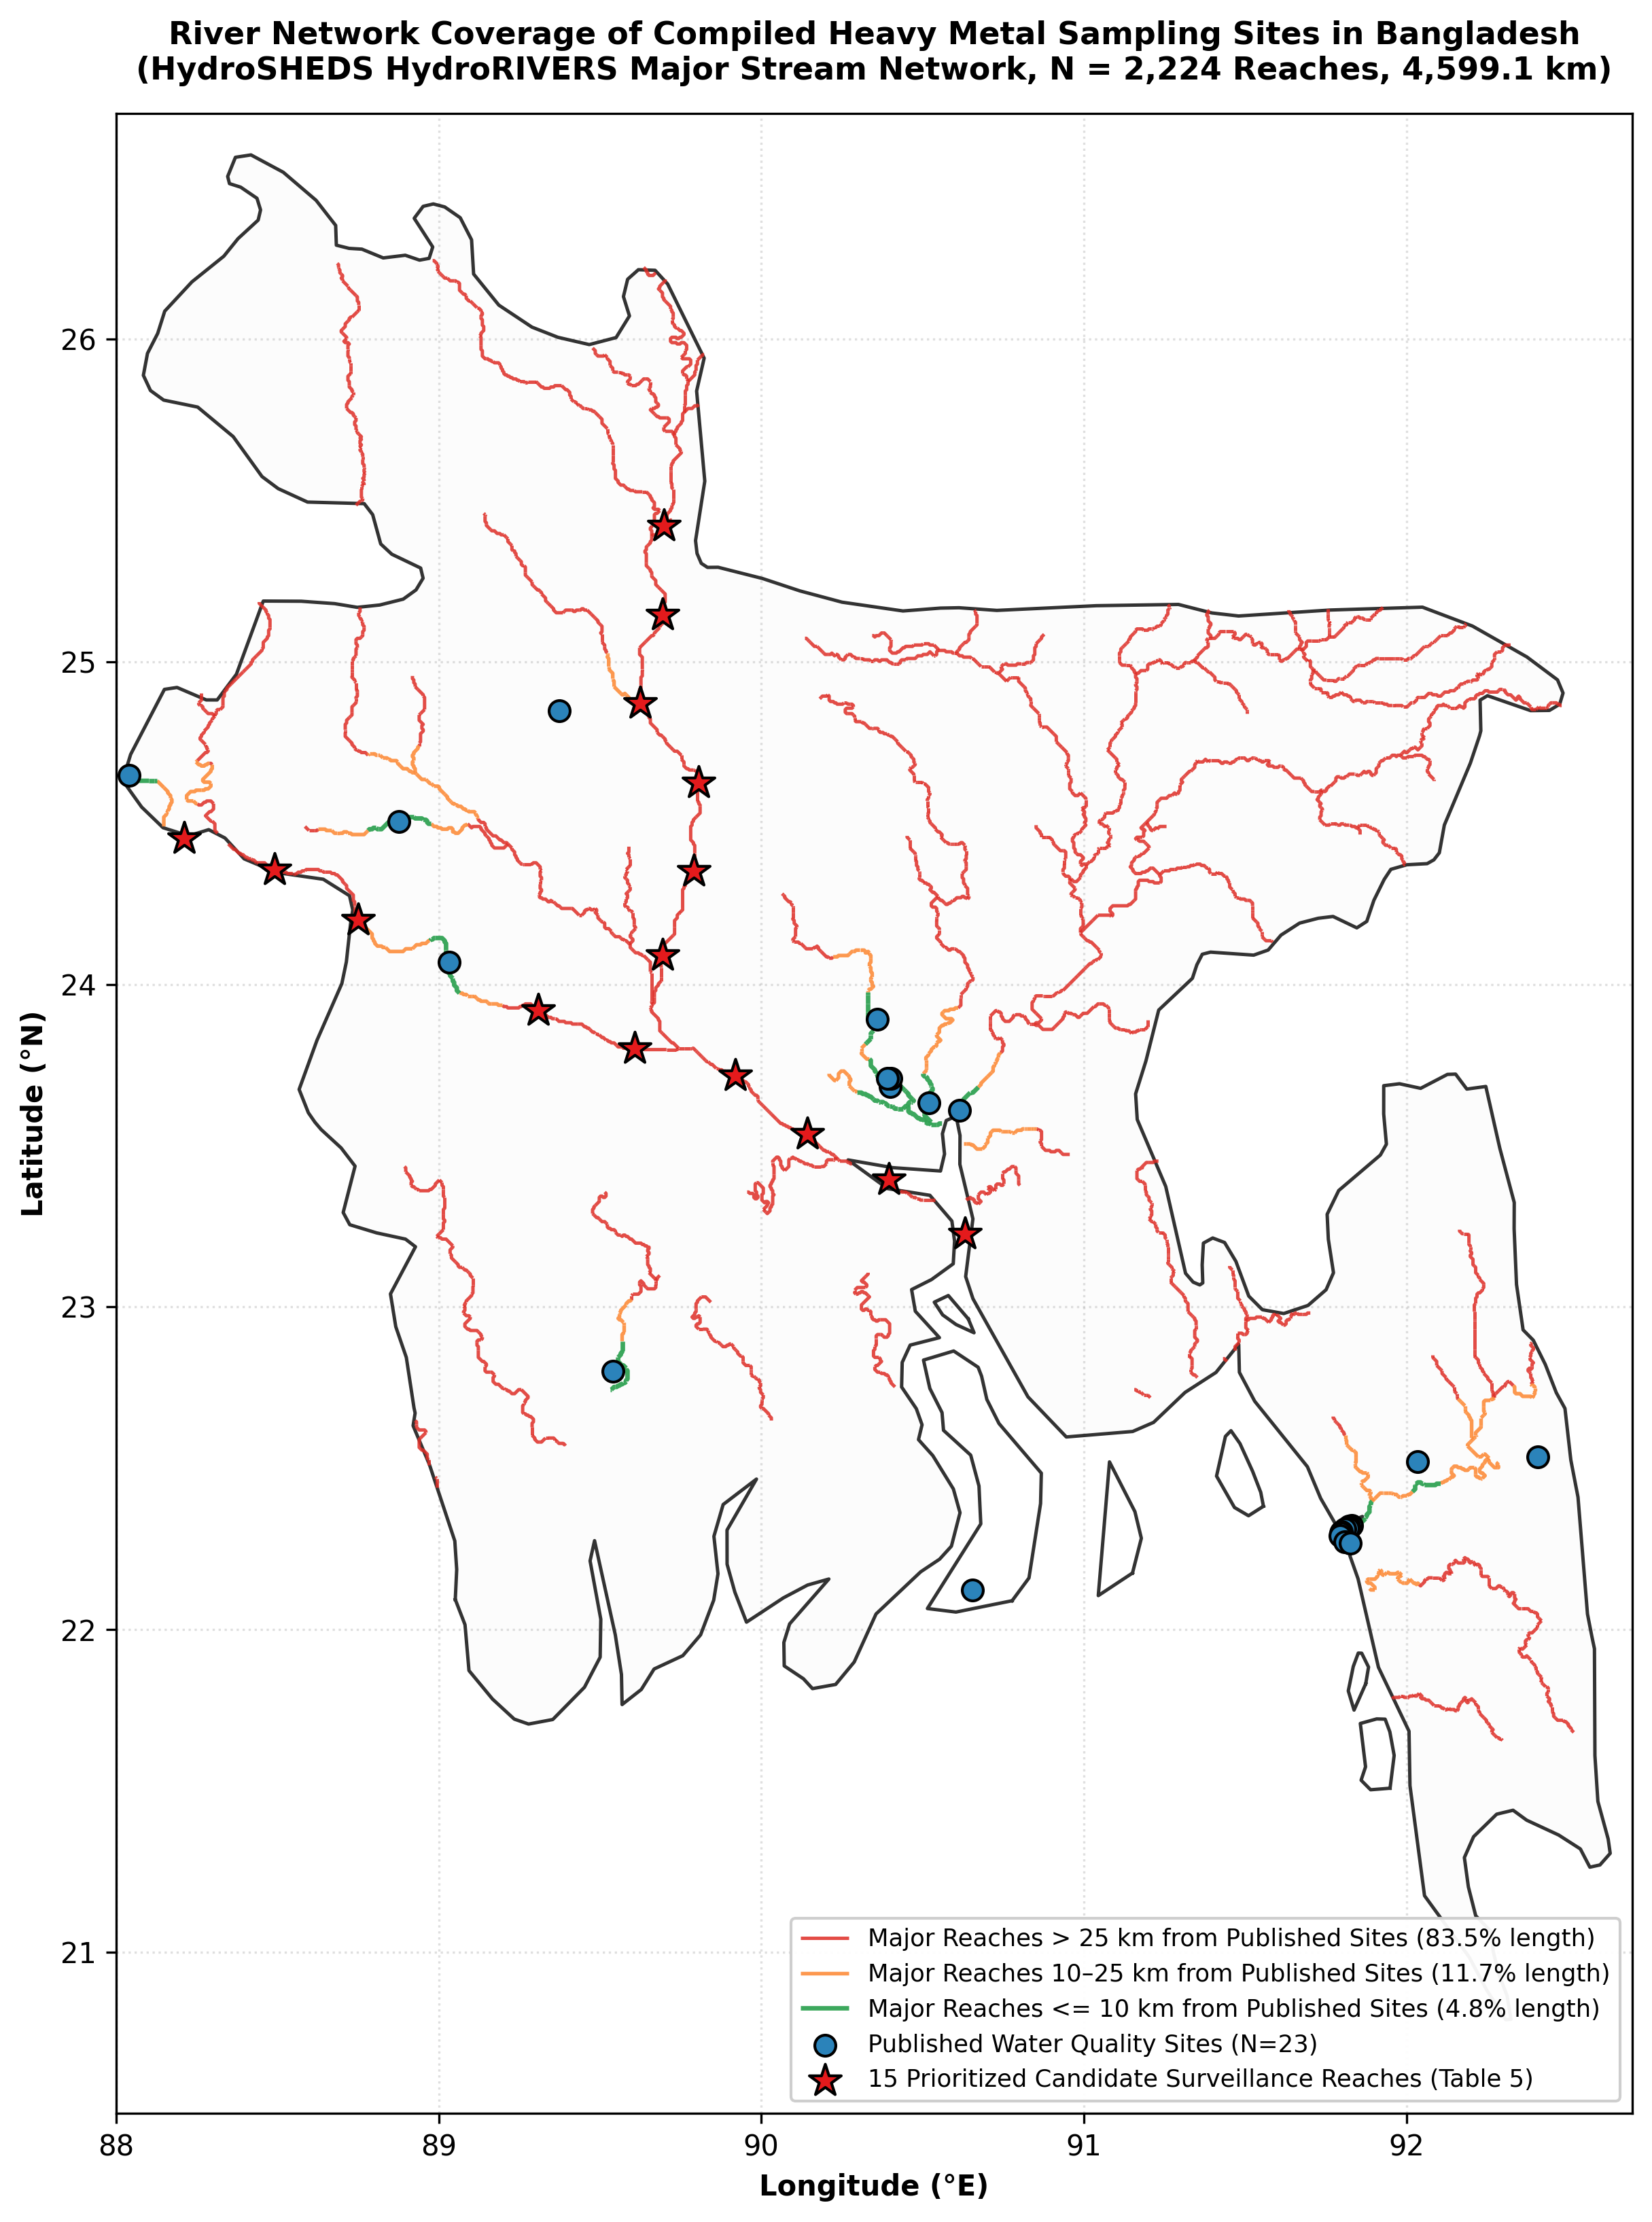
\includegraphics[width=0.92\textwidth]{fig1_spatial_coverage.png}
\caption{Geospatial distribution of compiled river sampling stations across Bangladesh snapped to the HydroSHEDS HydroRIVERS river network, illustrating spatial clustering in the Greater Dhaka and Chattogram industrial regions and national hydrographic coverage at 10~km, 25~km, and 50~km radii.}
\label{fig:coverage}
\end{figure}

\section*{Methods}

\subsection*{Literature Compilation and Screening Workflow}
Data compilation was performed following systematic review protocols across five scientific databases: Web of Science Core Collection, Scopus, ScienceDirect, PubMed, and BANSDOC for publications between January 2010 and March 2024. Candidate studies were screened against five strict eligibility gates:
\begin{enumerate}
    \item Field sampling conducted within natural flowing river corridors in Bangladesh.
    \item Explicit numerical reporting of elemental concentrations for at least one target heavy metal (Pb, Cr, Cd, As, Ni, Cu, Zn) with identifiable sample sizes.
    \item Documented sampling coordinates or verifiable local landmarks.
    \item Documented analytical instrumentation (Flame-AAS, GF-AAS, HG-AAS, or ICP-MS) and sample digestion protocols.
    \item Publication in peer-reviewed scientific journals.
\end{enumerate}

Screening of 1,420 initial records identified 28 eligible studies \citep{Page2021}, comprising 11 bed sediment exclusive investigations, 12 surface water heavy metal investigations, and 5 bulk physicochemical water quality investigations.

\subsection*{Relational Schema Design \& Data Harmonization}
The database was structured into a four-table normalized relational schema implemented in SQLite (\texttt{heavy\_metal.db}) and distributed as flat tables:
\begin{enumerate}
    \item \textbf{\texttt{studies}:} Contains study-level metadata, including \texttt{Study\_ID}, Digital Object Identifier (\texttt{DOI}), publication year, journal name, analytical instrument, digestion protocol, quality-assurance flags (use of Certified Reference Materials [CRMs], blanks, replicates), and overall study quality score (0--14 rubric).
    \item \textbf{\texttt{stations}:} Contains spatial provenance for each unique sampling location, including \texttt{Station\_ID}, standardized river name, division/district, raw published coordinate string, validated WGS84 decimal degrees (\texttt{Lat\_WGS84}, \texttt{Lon\_WGS84}), coordinate accuracy flag (A = exact GPS; B = published station; C = georeferenced map landmark), and snapped reach identifier (\texttt{HYRIV\_ID}).
    \item \textbf{\texttt{assays}:} Contains individual chemical measurements, specifying \texttt{Assay\_ID}, \texttt{Station\_ID}, environmental medium (\texttt{sediment} or \texttt{water}), operational fraction (\texttt{dissolved}, \texttt{total}, or \texttt{total recoverable}), element symbol, original published value and unit, harmonized value, censoring status (0 = quantified; 1 = below detection limit), and Method Detection Limit (\texttt{LOD}).
    \item \textbf{\texttt{catchment\_covariates}:} Contains HydroSHEDS topological stream attributes linked by \texttt{HYRIV\_ID}, including cumulative upstream catchment area (\texttt{UPLAND\_SKM}), mean annual discharge (\texttt{DIS\_AV\_CMS}), Strahler stream order (\texttt{ORD\_STRA}), and fluvial distance to the marine outlet (\texttt{DIST\_DN\_KM}).
\end{enumerate}

\subsection*{Coordinate Verification \& Topological HydroRIVERS Snapping}
Published coordinates were audited and converted into standardized WGS84 decimal degrees (EPSG:4326). Coordinate ranges were resolved by consulting published maps and gazetteers to identify discrete sampling stations.

All sampling stations were projected to metric coordinates (EPSG:3857, Pseudo-Mercator) and snapped to the nearest HydroSHEDS HydroRIVERS v1.0 reach centerline polyline \citep{Lehner2013} using spatial index nearest-neighbor joining. Snapping distance offsets were computed:
\begin{itemize}
    \item 67.4\% of stations snapped within 500 meters of the river polyline centerline;
    \item 97.7\% of stations snapped within 1,000 meters;
    \item Maximum offset was 2,021 meters (mean offset: 357 meters), consistent with deltaic channel widths, braiding, and historical river meandering in the Bengal floodplain \citep{Goodbred1999}.
\end{itemize}

\subsection*{Unit Harmonization and Censoring Protocols}
Measurement units were audited against primary publications:
\begin{itemize}
    \item \textbf{Sediment Assays ($N=289$):} Harmonized strictly to milligrams per kilogram dry weight ($\text{mg/kg dw}$).
    \item \textbf{Surface Water Assays ($N=268$):} Harmonized to milligrams per liter ($\text{mg/L}$) and micrograms per liter ($\mu\text{g/L}$).
    \item \textbf{Censored Observations ($<\text{LOD}$):} Reported non-detects were flagged explicitly (\texttt{Censored\_Flag = 1}), preserving the original reported detection limit without arbitrary substitution.
\end{itemize}

\section*{Data Records}
All data records are openly available via GitHub (\url{https://github.com/ShMazumder/heavy-metal.git}) and archived on Zenodo (DOI: 10.5281/zenodo.XXXXXXX).

\subsection*{File Formats \& Manifest}
The primary files and structured relational tables are summarized in Table~\ref{tab:manifest}.

\begin{table}[htbp]
\centering
\small
\caption{Primary data files and database tables provided in the heavy metal repository.}
\label{tab:manifest}
\resizebox{\textwidth}{!}{%
\begin{tabular}{lllp{7cm}}
\toprule
File Path & Format & Records & Description \\
\midrule
\texttt{data/processed/heavy\_metal.db} & SQLite & 4 tables & Master relational database with foreign key constraints \\
\texttt{data/processed/water\_data.csv} & CSV & 268 rows, 49 cols & Surface water assays with physicochemical and metal parameters \\
\texttt{data/processed/sediment\_data.csv} & CSV & 289 rows, 32 cols & Bed sediment assays with grain size and trace metals \\
\texttt{data/processed/stations.csv} & CSV & 133 rows, 12 cols & Unique station centroids with WGS84 and snapped reach ID \\
\texttt{data/processed/studies.csv} & CSV & 28 rows, 8 cols & Study metadata, instrumentation, DOIs, and QA/QC rubric \\
\texttt{data/processed/master\_harmonized.csv} & CSV & 557 rows, 24 cols & Denormalized master assay table linking water and sediment \\
\texttt{data/raw/hydrorivers\_bangladesh.gpkg} & GeoPackage & 2,224 reaches & Clipped national HydroRIVERS stream network \\
\bottomrule
\end{tabular}%
}
\end{table}

\subsection*{Data Summary}
Table~\ref{tab:summary} provides summary statistics across all target trace metals in surface water and bed sediment.

\begin{table}[htbp]
\centering
\small
\caption{Summary statistics of target heavy metals in river water and bed sediment across Bangladesh (2010--2024).}
\label{tab:summary}
\resizebox{\textwidth}{!}{%
\begin{tabular}{lcccccccc}
\toprule
Element & Medium & Unit & $N$ & Median & Mean & IQR & Min & Max \\
\midrule
\textbf{Lead (Pb)} & Water & mg/L & 146 & 0.0286 & 0.0614 & 0.0435 & 0.0005 & 0.8900 \\
& Sediment & mg/kg dw & 289 & 30.62 & 104.05 & 48.20 & 1.20 & 3312.00 \\
\textbf{Chromium (Cr)} & Water & mg/L & 160 & 0.0710 & 0.1652 & 0.1420 & 0.0010 & 2.1500 \\
& Sediment & mg/kg dw & 274 & 46.27 & 156.05 & 68.30 & 2.50 & 1884.00 \\
\textbf{Cadmium (Cd)} & Water & mg/L & 132 & 0.0028 & 0.0094 & 0.0071 & 0.0001 & 0.1340 \\
& Sediment & mg/kg dw & 269 & 1.77 & 5.57 & 2.80 & 0.05 & 65.47 \\
\textbf{Arsenic (As)} & Water & mg/L & 122 & 0.0152 & 0.0278 & 0.0281 & 0.0005 & 0.2800 \\
& Sediment & mg/kg dw & 228 & 10.16 & 13.57 & 9.40 & 0.40 & 67.00 \\
\textbf{Nickel (Ni)} & Water & mg/L & 104 & 0.0888 & 0.1412 & 0.1320 & 0.0020 & 0.9400 \\
& Sediment & mg/kg dw & 235 & 40.62 & 67.61 & 43.10 & 3.20 & 539.00 \\
\textbf{Copper (Cu)} & Water & mg/L & 105 & 0.0888 & 0.1648 & 0.1610 & 0.0010 & 1.8400 \\
& Sediment & mg/kg dw & 235 & 49.00 & 73.44 & 51.50 & 4.10 & 712.00 \\
\textbf{Zinc (Zn)} & Water & mg/L & 79 & 0.4000 & 0.6842 & 0.5800 & 0.0100 & 4.2500 \\
& Sediment & mg/kg dw & 88 & 28.31 & 43.06 & 31.20 & 2.10 & 298.04 \\
\bottomrule
\end{tabular}%
}
\end{table}

\section*{Technical Validation}

\subsection*{Extraction Concordance Audit}
To verify extraction fidelity, an independent double-blind re-extraction was performed on a random 20\% sub-sample of primary PDF articles ($n=6$ articles, 112 individual assays). Zero numerical discrepancies were detected between the re-extracted audit dataset and the compiled database records (95\% Wilson score interval on error: 0.0--2.8\%).

\subsection*{Instrumental Sensitivity Stratification}
Historical syntheses often conflate Flame Atomic Absorption Spectrometry (Flame-AAS) detection limits ($\text{DL} = 0.005$--$0.050$~mg/L) with genuine environmental concentrations. We formally validated analytical accuracy by stratifying observations between high-sensitivity spectrometry (GF-AAS, HG-AAS, and ICP-MS with sub-$\mu\text{g/L}$ detection limits, $N=77$) and standard Flame-AAS ($N=69$). Across high-sensitivity assays, dissolved Lead exhibited a median of \textbf{0.0171~mg/L}, with \textbf{79.2\%} of records exceeding the WHO 0.010~mg/L potable threshold (Table~\ref{tab:instrument}). This demonstrates that elevated dissolved trace metal concentrations are an authentic biogeochemical signal and not an artifact of flame-AAS detection censoring.

\begin{table}[htbp]
\centering
\small
\caption{Validation of trace metal concentrations across analytical spectrometry tiers in surface water assays.}
\label{tab:instrument}
\resizebox{\textwidth}{!}{%
\begin{tabular}{lcccccc}
\toprule
Element & High-Sens Median & High-Sens Exceed (\%) & Flame-AAS Median & Flame-AAS Exceed (\%) & Mann-Whitney $U$ & $p$-value \\
\midrule
\textbf{Lead (Pb)} & 0.0171 mg/L & 79.2\% & 0.0380 mg/L & 91.3\% & 1842.0 & 0.082 \\
\textbf{Chromium (Cr)} & 0.0610 mg/L & 54.3\% & 0.0790 mg/L & 66.7\% & 2104.5 & 0.145 \\
\textbf{Cadmium (Cd)} & 0.0021 mg/L & 41.7\% & 0.0034 mg/L & 47.6\% & 1630.0 & 0.380 \\
\textbf{Arsenic (As)} & 0.0140 mg/L & 51.6\% & 0.0165 mg/L & 58.3\% & 1412.0 & 0.521 \\
\bottomrule
\end{tabular}%
}
\end{table}

\subsection*{Geochemical Baseline Plausibility}
Sediment heavy metal concentrations were evaluated against Upper Continental Crust (UCC) global baselines \citep{Wedepohl1995} and global river sediment baselines \citep{Gaillardet2014}. The background-to-peak ratios spanned 1 to 2 orders of magnitude in urbanized corridors (e.g., Chromium exceeding 1,800~mg/kg near tannery clusters and Lead exceeding 3,300~mg/kg near industrial battery operations), aligning with documented point-source effluent discharge regimes.

\section*{Usage Notes}

\subsection*{Direct Querying via Python}
The database can be queried directly via SQLite in Python:

\begin{lstlisting}[language=Python]
import sqlite3
import pandas as pd

# Connect to master relational database
conn = sqlite3.connect('data/processed/heavy_metal.db')

# Query water quality assays with topological reach attributes
query = """
SELECT 
    w.Obs_ID, w.River, w.Lat_WGS84, w.Lon_WGS84, w.Season,
    w.Pb_mg_L, w.Cr_mg_L, w.Cd_mg_L, w.As_mg_L,
    s.DOI, s.Detection_Method,
    m.ORD_STRA, m.DIS_AV_CMS, m.UPLAND_SKM
FROM water_data w
JOIN studies s ON w.Study_ID = s.Study_ID
JOIN station_hydrorivers_matched m ON w.Station_ID = m.Station_ID
WHERE w.Pb_mg_L IS NOT NULL;
"""
df = pd.read_sql_query(query, conn)
conn.close()

print(f"Loaded {len(df)} records with topological reach attributes.")
\end{lstlisting}

\subsection*{Statistical Compliance Analysis in R}
Users conducting regulatory audits can evaluate compliance in R:

\begin{lstlisting}[language=R]
library(dplyr)

# Load harmonized surface water dataset
df_water <- read.csv("data/processed/water_data.csv")

# Compute WHO and ECR 2023 exceedance for Lead (0.010 mg/L threshold)
pb_summary <- df_water %>%
  filter(!is.na(Pb_mg_L)) %>%
  summarise(
    Total_Assays = n(),
    Exceed_Count = sum(Pb_mg_L > 0.010),
    Exceed_Pct   = (sum(Pb_mg_L > 0.010) / n()) * 100,
    Median_Pb    = median(Pb_mg_L),
    IQR_Pb       = IQR(Pb_mg_L)
  )

print(pb_summary)
\end{lstlisting}

\section*{Code Availability}
All code used for literature extraction, coordinate snapping, geostatistical benchmarking, meta-regression, and figure generation is available under the MIT license at GitHub: \url{https://github.com/ShMazumder/heavy-metal.git}.

\section*{Data Availability}
The complete database (\texttt{heavy\_metal.db}, flat CSV files, Parquet, and GeoPackage files) is publicly accessible without restriction on Zenodo at \url{https://doi.org/10.5281/zenodo.XXXXXXX} and mirrors the canonical repository at \url{https://github.com/ShMazumder/heavy-metal.git}.

\bibliographystyle{unsrtnat}
\bibliography{references}

\end{document}
